% !TEX root = ../thesis.tex

\chapter{Erstellung eines featurebasierten Datensets}
\label{dataset-creation}

Dieses Kapitel widmet sich der schrittweisen Erläuterung des Prozesses zur Erstellung des featurebasierten Datensets, welches zur Anlernung der Machine-Learning-Klassifikatoren dient. Dazu wird zunächst die Datenauswahl näher beleuchtet. Darauf folgt eine Darlegung der Konstruktion des Datensets sowie der Auswahl und Berechnung der Metriken, welche als Attribute im Rahmen der Anlernung der Klassifikatoren dienen. Eine Gliederung der Kapitel kann \autoref{fig:kap3} entnommen werden.

\begin{figure}[H]
    \centering
    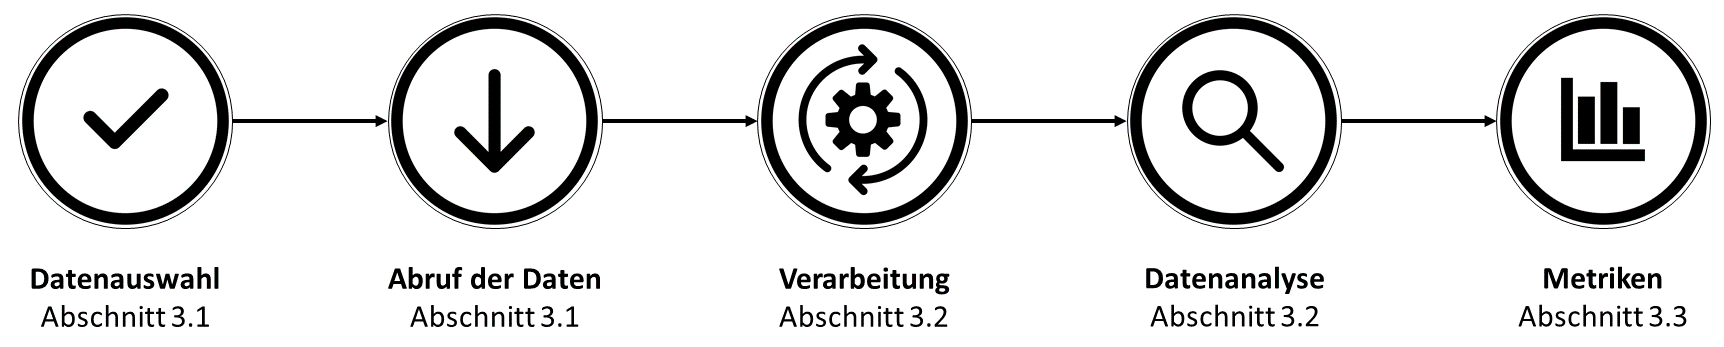
\includegraphics[width=\textwidth]{images/Kap3}
    \caption{Übersicht zur Gliederung des dritten Kapitels\label{fig:kap3}}
\end{figure}

\hrule

\section{Datenauswahl}

Wie im vorangegangenen Kapitel bereits erwähnt wurde, bildet das Datenset die Grundlage für die Anlernung der Machine-Learning-Klassifikatoren und wird eigens für diese Arbeit auf Basis von Commits-Daten von 13 featurebasierten Softwareprojekten erstellt. Die Auswahl der Softwareprojekte erfolge anhand von vorheriger Verwendung in wissenschaftlicher Literatur \cite{Hunsen2015,Liebig2010,Queiroz2015,Queiroz2016}. Die für diese Arbeit verwendeten Softwareprojekte sind samt ihres Einsatzzweckes und ihrer Datenquellen in \autoref{tab:tools} aufgeführt.

\begin{table}[t]
\centering
\caption{Übersicht der verwendeten Softwareprojekte\protect\footnotemark{}}
\label{tab:tools}
\resizebox{\linewidth}{!}{%
\begin{tabular}{|l|l|l|l|l|l|l|} 
\cline{1-3}\cline{5-7}
\textbf{Projekt}   & \textbf{Zweck}       & \textbf{Datenquelle}  & ~                    & \textbf{Projekt}     & \textbf{Zweck}       & \textbf{Datenquelle}                     \\ 
\cline{1-3}\cline{5-7}
\textbf{Blender}   & 3D-Modellierungstool & GitHub-Mirror         & ~                    & \textbf{libxml2}     & XML-Parser           & GitLab-Repository                        \\ 
\cline{1-3}\cline{5-7}
\textbf{Busybox}   & UNIX-Toolkit         & Git-Repository        & ~                    & \textbf{lighttpd}    & Webserver            & Git-Repository                           \\ 
\cline{1-3}\cline{5-7}
\textbf{Emacs}     & Texteditor           & GitHub-Mirror         & ~                    & \textbf{MPSolve}     & Polynomlöser         & GitHub-Repository                        \\ 
\cline{1-3}\cline{5-7}
\textbf{GIMP}      & Bildbearbeitung      & GitLab-Repository     & ~                    & \textbf{Parrot}      & virtuelle Maschine   & GitHub-Repository                        \\ 
\cline{1-3}\cline{5-7}
\textbf{Gnumeric}  & Tabellenkalkulation  & GitLab-Repository     & ~                    & \textbf{Vim}         & Texteditor           & GitHub-Repository                        \\ 
\cline{1-3}\cline{5-7}
\textbf{gnuplot}   & Plotting-Tool        & GitHub-Mirror         & ~                    & \textbf{xfig}        & Grafikeditor         & Sourceforge-Repository  \\ 
\cline{1-3}\cline{5-7}
\textbf{Irssi}     & IRC-Client           & GitHub-Repository     & \multicolumn{1}{l}{} & \multicolumn{1}{l}{} & \multicolumn{1}{l}{} & \multicolumn{1}{l}{}                     \\
\cline{1-3}
\end{tabular}
}
\end{table}
\footnotetext{Links zu den Websites der Softwareprojekte und deren Repositories können im \hyperref[appendix1]{Anhang} eingesehen werden.}

Um die Commit-Daten der Softwareprojekte zu erhalten wurde die Python-Library PyDriller\footnote{\href{https://github.com/ishepard/pydriller}{https://github.com/ishepard/pydriller}} verwendet \cite{Spadini2018}. Diese ermöglicht eine einfache Datenextraktion aus Git-Repositories zum Erhalt von Commits, Commit-Nachrichten, Entwicklern, Diffs und mehr (im weiteren Verlauf \glqq Metadaten\grqq{} genannt). Ein beispielhafter Sourcecode-Ausschnitt zur Konsolenausgabe von Metadaten eines Commits (Autor, Name der veränderten Dateien, Typ der Veränderung und jeweilige zyklomatische Komplexität der Dateien) ist in \autoref{pydriller} aufgeführt. 

\begin{lstlisting}[language=Python, caption=Beispielhafter PyDriller-Code zur Ausgabe von Metadaten von Commits, frame=single, label=pydriller]
for commit in RepositoryMining("link_to_repo").traverse_commits(): 
	for m in commit.modifications: 
		print( 
		     "Author {}".format(commit.author.name), 
		     " modified {}".format(m.filename), 
		     " with a change type of {}".format(m.change_type.name), 
		     " and the complexity is {}".format(m.complexity) 
		)
\end{lstlisting}

Als Input der eigens erstellten Python-Scripte zum Erhalt der Commit-Metadaten dienten jeweils die URLs zu den Git-Repositories der Softwareprojekte. Weiterhin wurden die Metadaten in Commits je Release aufgeteilt. Ermöglicht wurde dies durch die Angabe von Release-Tags im PyDriller-Code, basierend auf der Tag-Struktur von Git-Repositories. Für jede veränderte Datei innerhalb eines Commits und eines Releases wurden die folgenden Metadaten mit Hilfe von PyDriller abgerufen:

\begin{multicols}{2}
\begin{itemize}
\setlength{\itemsep}{-2pt}
\item Commit-Hash (eindeutiger Bezeichner des zugehörigen Commits)
\item Autor des zugehörigen Commits
\item zugehörige Commit-Nachricht
\item Name der veränderten Datei
\item Lines-of-Code der veränderten Datei
\item zyklomatische Komplexität der veränderten Datei
\item Anzahl der hinzugefügten Zeilen zur Datei
\item Anzahl der entfernten Zeilen von der Datei
\item Art der Änderung (ADD, REM, MOD)\footnote{Diese Information fand in der weiteren Erstellung des Datensets keine Verwendung.}
\item Diff (Changeset) der Veränderung
\item[\vspace{\fill}]
\end{itemize}
\end{multicols}

Die auf diese Weise erhaltenen Daten wurden nach dem Abruf in einer MySQL-Datenbank gespeichert. Für jedes Softwareprojekt wurde eine eigene Tabelle erstellt, in welcher neben der oben stehenden Metadaten zudem der Name des betreffenden Softwareprojekts und die den Commits zugehörigen Release-Nummern gespeichert wurden. Jede veränderte Datei eines Commits erhält eine Zeile der Datenbank-Tabellen. In \autoref{tab:tools-values1} kann eingesehen werden, wie viele Releases je Softwareprojekt abgerufen wurden und wie viele Commits daraus resultieren.

\begin{table}[t]
\centering
\caption{Übersicht der Anzahl der Releases und Commits je Softwareprojekt}
\label{tab:tools-values1}
\resizebox{\linewidth}{!}{%
\begin{tabular}{|>{\hspace{0pt}}p{0.152\linewidth}|>{\RaggedLeft\hspace{0pt}}p{0.158\linewidth}|>{\RaggedLeft\hspace{0pt}}p{0.156\linewidth}|>{\hspace{0pt}}p{0.029\linewidth}|>{\hspace{0pt}}p{0.139\linewidth}|>{\RaggedLeft\hspace{0pt}}p{0.168\linewidth}|>{\RaggedLeft\hspace{0pt}}p{0.185\linewidth}|} 
\cline{1-3}\cline{5-7}
\textbf{Projekt}   & \textbf{\#Releases}  & \textbf{\#Commits}  & ~                                                     & \textbf{Projekt}                                     & \textbf{\#Releases}~                                 & \textbf{\#Commits}~ ~                                 \\ 
\cline{1-3}\cline{5-7}
\textbf{Blender}   & 11                   & 19.119              & ~                                                     & \textbf{libxml2}                                     & 10                                                   & 732                                                   \\ 
\cline{1-3}\cline{5-7}
\textbf{Busybox}   & 14                   & 4.984               & ~                                                     & \textbf{lighttpd}                                    & 6                                                    & 2.597                                                 \\ 
\cline{1-3}\cline{5-7}
\textbf{Emacs}     & 7                    & 12.805              & ~                                                     & \textbf{MPSolve}                                     & 8                                                    & 668                                                   \\ 
\cline{1-3}\cline{5-7}
\textbf{GIMP}      & 14                   & 7.240               & ~                                                     & \textbf{Parrot}                                      & 7                                                    & 16.245                                                \\ 
\cline{1-3}\cline{5-7}
\textbf{Gnumeric}  & 8                    & 6.025               & ~                                                     & \textbf{Vim}                                         & 7                                                    & 9.849                                                 \\ 
\cline{1-3}\cline{5-7}
\textbf{gnuplot}   & 5                    & 6.619               & ~                                                     & \textbf{xfig}                                        & 7                                                    & 18                                                    \\ 
\cline{1-3}\cline{5-7}
\textbf{Irssi}     & 7                    & 253                 & \multicolumn{1}{>{\hspace{0pt}}p{0.029\linewidth}}{~} & \multicolumn{1}{>{\hspace{0pt}}p{0.139\linewidth}}{} & \multicolumn{1}{>{\hspace{0pt}}p{0.168\linewidth}}{} & \multicolumn{1}{>{\hspace{0pt}}p{0.185\linewidth}}{}  \\
\cline{1-3}
\end{tabular}
}
\end{table}

Diese \glqq Rohdaten\grqq{} dienen zur weiteren Verarbeitung hinsichtlich der Erstellung des Datensets und der anschließenden Berechnung der Metriken. Eine Erläuterung der weiteren Verarbeitung der Daten folgt im kommenden Abschnitt.

\fbox{\parbox{\linewidth}{RQ1a: WELCHE DATEN KOMMEN FÜR DIE ERSTELLUNG DES DATENSETS IN FRAGE?\medskip\\
Es kommen die Daten von 13 featurebasierten Softwareprojekten zur Verwendung. Mithilfe der Python-Library PyDriller wurden die Metadaten der Commits, aufgeteilt nach Commits pro Release, aus den Git-Repositories extrahiert und in MySQL-Datenbanken gespeichert. Ausgewählt wurden die Softwareprojekte aufgrund einer vorherigen Verwendung in der wissenschaftlichen Literatur \cite{Hunsen2015,Liebig2010,Queiroz2016}.}}

\section{Konstruktion des Datensets}
\label{construction}

Die Konstruktion des Datensets gliedert sich in mehrere Phasen der Datenverarbeitung und -optimierung. Diese werden im folgenden vorgestellt.

\subsection*{Identifikation von Features}

Die erste Phase besteht aus der Extraktion der involvierten Features einer veränderten Datei. Dazu wurden mithilfe eines Python-Scripts die Präprozessor-Anweisungen \texttt{\#IFDEF} und \texttt{\#IFNDEF} in den Diffs der veränderten Dateien identifiziert und anschließend die den Direktiven folgende Zeichenfolge bis zum Ende der Codezeile als Feature gespeichert. Die Identifizierung erfolgte mittels regulären Ausdrücken. Gespeichert werden die je Datei identifizierten Features in einer zusätzlichen Spalte in den jeweiligen MySQL-Tabellen der Metadaten der Softwareprojekte. Für den Fall, dass ein Feature hinter der Direktive \texttt{\#IFNDEF} identifiziert wurde, wird das Feature mit einem vorangestellten \glqq not\grqq{} gespeichert. Es wird somit als eigenständiges Feature, neben seiner nicht-negierten Form, gespeichert. Kombinationen von Features werden in ihrer identifizierten Form gespeichert. Konnte kein Feature identifiziert werden, wird entsprechend \glqq \texttt{none}\grqq{} gespeichert.

Dieser Weg der Identifizierung birgt einige Hindernisse. Diese können, neben dem Normalfall, in \autoref{fig:features} gesehen werden. In einigen C-Programmierparadigmen ist es üblich, Header-Dateien mittels Präprozessor-Direktiven im Sourcecode einzubinden, sodass sie wie Features scheinen (siehe erster unerwünschter Fall in \autoref{fig:features}). Diese \glqq Header-Features\grqq{}, wie sie im weiteren Verlauf genannt werden, sollten jedoch ignoriert werden, da sie im gesamten Sourcecode keine Variabilität erzeugen. In der Regel sind diese Header-Features identifizierbar durch ihre Namensgebung in Form eines angehängten \texttt{\_h\_} an den Featurenamen, wie beispielsweise \texttt{featurename\_h\_}. Dieser angehängte Teil erlaubt es, die Header-Features mittels regulärer Ausdrücke zu erkennen und auszufiltern. 

Ebenfalls besteht die Möglichkeit, dass \glqq falsche\grqq{} Features identifiziert werden können. Beispiele dafür können von \texttt{\#IFDEFs} stammen, welche in Kommentaren verwendet wurden (siehe zweiter unerwünschter Fall in \autoref{fig:features}). Solche falschen Features wurden in einer manuellen Sichtung der identifizierten Features entfernt und durch \glqq \texttt{none}\grqq{} ersetzt.

\begin{figure}[t]
    \centering
    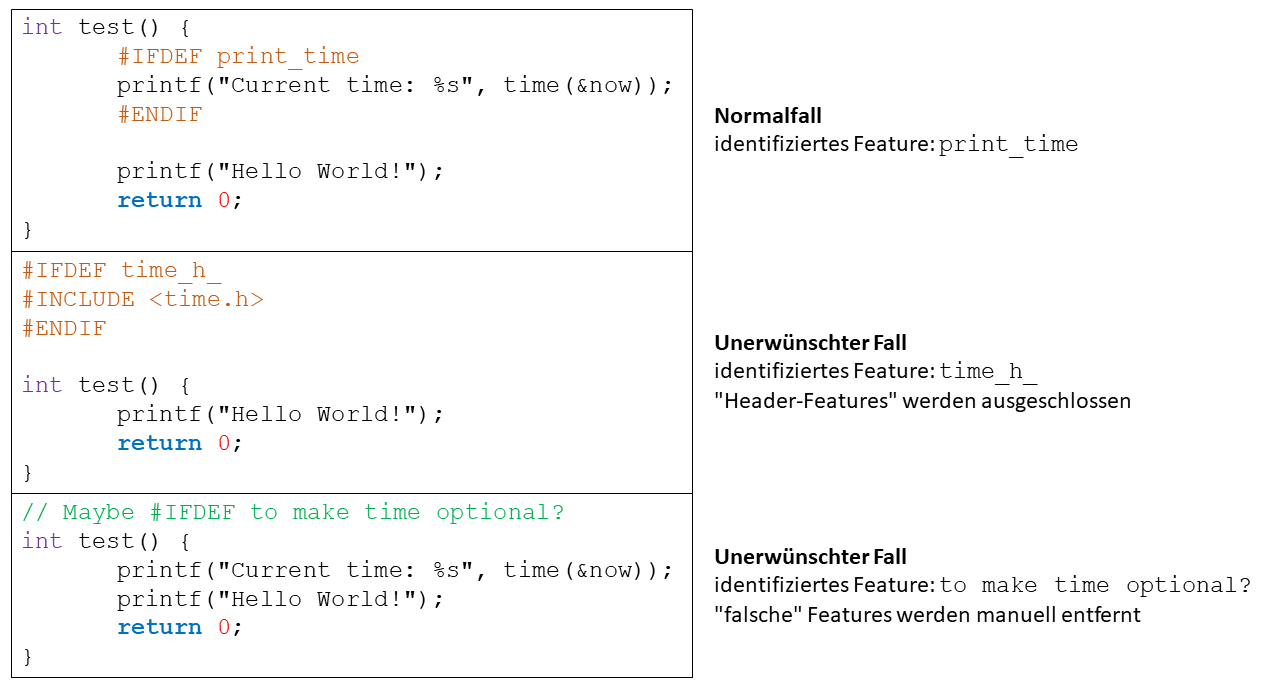
\includegraphics[width=\textwidth]{images/Features}
    \caption{Normalfall und unerwünschte Fälle bei der Identifizierung der Features\label{fig:features}}
\end{figure}

\subsection*{Identifikation von korrektiven Commits}

Die nächste Phase der Verarbeitung besteht aus der Identifizierung von korrektiven Commits. Eine dafür gängige Methode, die auch in dieser Arbeit Anwendung fand, besteht aus der Analyse der Commit-Nachrichten auf das Vorhandensein von bestimmten Schlagwörtern \cite{Zimmermann2007}. Bei den Schlagwörtern handelt es sich um \glqq bug\grqq,\glqq bugs\grqq{}, \glqq bugfix\grqq{}, \glqq error\grqq, \glqq fail\grqq{}, \glqq fix\grqq, \glqq fixed\grqq{} und \glqq fixes\grqq. Durchgeführt wurde die Analyse mittels eines Python-Skripts unter Zuhilfenahme von einfachen Methoden des Natural Language Processings (NLP). Dabei wurde die Identifizierung auf die jeweils erste Zeile der Commit-Nachrichten beschränkt. Die Ergebnisse wurden in einer weiteren Spalte der MySQL-Tabellen (true = korrektiv, false = nicht korrektiv) gespeichert.

\subsection*{Identifikation fehlereinführender Commits}
\label{szz-def}
Der Suche nach korrektiven Commits folgt eine Analyse nach fehlereinführenden Commits. Dazu wurde eine PyDriller-Implementierung des SZZ-Algorithmus nach Sliwerski, Zimmermann und Zeller verwendet \cite{Sliwerski2005,Spadini2018}. Dieser Algorithmus erlaubt es fehlereinführende Commits in lokal gespeicherten Software-Repositories zu finden \cite{Borg2019}. Dafür setzt er voraus, dass die korrektiven Commits bereits identifiziert wurden, da sie als Eingabemenge des Algorithmus dienen \cite{Borg2019}. Die Identifikation der fehlereinführenden Commits ist in mehrere Schritte unterteilt und wird in \autoref{fig:szz} dargestellt. Die Erläuterungen der mit Buchstaben versehenen Schritte erfolgt im Anschluss. Die für diese Arbeit verwendete PyDriller-Implementierung des Algorithmus folgt dem gezeigten Ablauf.

\begin{figure}[t]
    \centering
    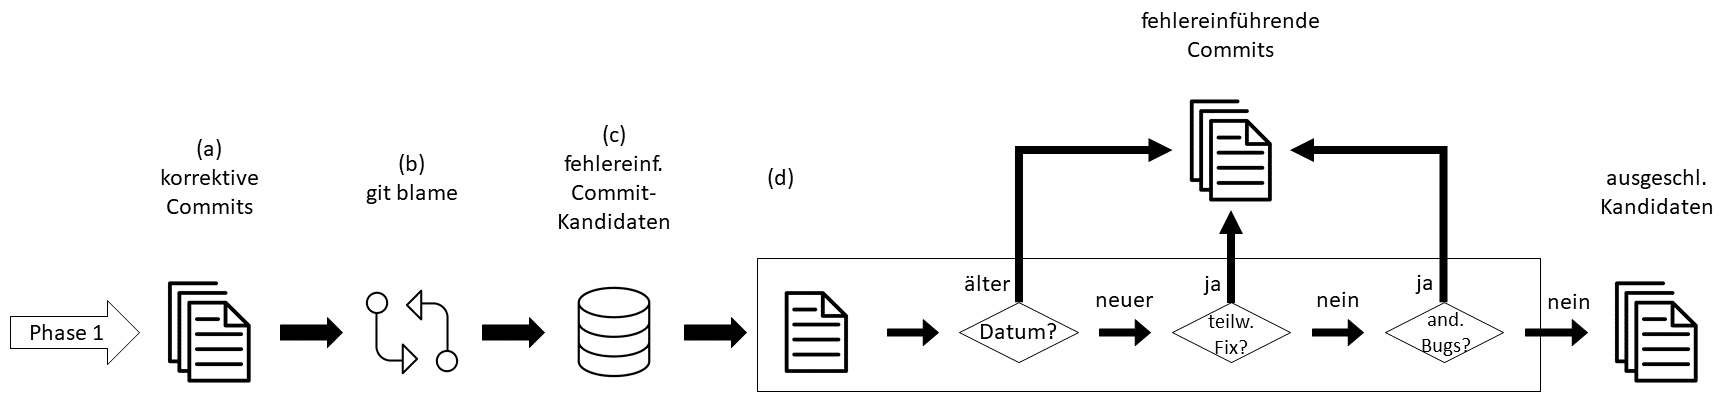
\includegraphics[width=\textwidth]{images/SZZ}
    \caption{Ablauf der zweiten Phase des SZZ-Algorithmus (übersetzt, \cite{Borg2019})\label{fig:szz}}
\end{figure}

Der SZZ-Algorithmus, der als Input eine Liste der Commit-Hashes der zuvor erkannten korrektiven Commits (a) erhält, beginnt mit der Ausführung eines \texttt{git blame} Befehls (b) zur Identifizierung sämtlicher Commits, in denen Veränderungen an den selben Dateien und Codezeilen vorgenommen wurden wie in den korrektiven Commits \cite{Borg2019}. Daraus resultieren mögliche fehlereinführende Commit-Kandidaten (c). Für jeden dieser Commit-Kandidaten wird dann erörtert, ob er fehlereinführend ist (d). Dazu wird zunächst das Datum des Commit-Kandidaten mit dem zugehörigen korrektiven Commits verglichen. Liegt dieses vor dem Datum des korrektiven Commits, so gilt der Kandidat als tatsächlich fehlereinführend \cite{Borg2019}. Liegt das Datum danach, so kann der Kandidat nur fehlereinführend sein, sofern er teilweise den vorhandenen Fehler löst (teilweiser Fix) oder für einen anderen Fehler verantwortlich ist, der nicht dem korrektiven Commit zugehörig ist (Kandidat ist Fehlerursache eines anderen korrektiven Commits) \cite{Borg2019}. Die Ausgabe ist eine Liste von Commit-Hashes von fehlereinführenden Commits für jede Datei eines korrektiven Commits. Diese neuen Informationen werden in einer zusätzlichen Spalte in den MySQL-Tabellen für jeden Eintrag gespeichert (true = fehlereinführend, false = nicht fehlereinführend). 

Eine Übersicht der Anzahl der korrektiven und fehlereinführenden Commits sowie der Anzahl der identifizierten Features je Softwareprojekt ist in \autoref{tab:tools-values2} aufgeführt. Des weiteren ist eine Übersicht des Schemas der nun vollständigen initialen MySQL-Tabellen (im folgenden Haupttabellen genannt) in \autoref{tab:schema1} aufgeführt. Wie bereits zuvor erwähnt, umfasst diese Tabelle für jede veränderte Datei eines Commits eine Ziele. Sollten in einem Diff einer veränderten Datei mehrere Features identifiziert worden sein, so wird für jedes Feature die entsprechende Zeile dupliziert.

\begin{table}
\centering
\caption{Anzahl der korrektiven und fehlereinführenden Commits sowie Anzahl der identifizierten Features je Softwareprojekt}
\label{tab:tools-values2}
\resizebox{\linewidth}{!}{%
\begin{tabular}{|>{\hspace{0pt}}p{0.208\linewidth}|>{\RaggedLeft\hspace{0pt}}p{0.21\linewidth}|>{\RaggedLeft\hspace{0pt}}p{0.362\linewidth}|>{\RaggedLeft\hspace{0pt}}p{0.212\linewidth}|} 
\hline
 \textbf{Projekt}  & \textbf{\#korrektiv}  & \textbf{\#fehlereinführend}  & \textbf{\#Features}   \\ 
\hline
\textbf{Blender}   & 7.760                 & 3.776                        & 1.400                 \\ 
\hline
\textbf{Busybox}   & 1.236                 & 802                          & 628                   \\ 
\hline
\textbf{Emacs}     & 4.269                 & 2.532                        & 718                   \\ 
\hline
\textbf{GIMP}      & 1.380                 & 854                          & 204                   \\ 
\hline
\textbf{Gnumeric}  & 1.498                 & 1.191                        & 637                   \\ 
\hline
\textbf{gnuplot}   & 854                   & 1.215                        & 558                   \\ 
\hline
\textbf{Irssi}     & 52                    & 22                           & 9                     \\ 
\hline
\textbf{libxml2}   & 324                   & 88                           & 200                   \\ 
\hline
\textbf{lighttpd}  & 1.078                 & 929                          & 230                   \\ 
\hline
\textbf{MPSolve}   & 151                   & 211                          & 54                    \\ 
\hline
\textbf{Parrot}    & 3.109                 & 3.072                        & 397                   \\ 
\hline
\textbf{Vim}       & 371                   & 696                          & 1.158                 \\ 
\hline
\textbf{xfig}      & 0*                    & 0*                           & 137                   \\ 
\hline
\multicolumn{4}{|>{\Centering\hspace{0pt}}p{0.992\linewidth}|}{* Siehe \hyperref[xfig]{Abschnitt 5.1}}             \\
\hline
\end{tabular}
}
\end{table}

\begin{table}[t]
\centering
\caption{Übersicht des Schemas der MySQL-Haupttabellen}
\label{tab:schema1}
\resizebox{\linewidth}{!}{%
\begin{tabular}{|>{\hspace{0pt}}p{0.25\linewidth}|>{\hspace{0pt}}p{0.746\linewidth}|} 
\hline
 \textbf{Spaltenname}  & \textbf{Beschreibung}                                     \\ 
\hline
name                   & Name des Softwareprojekts                                 \\ 
\hline
release\_number        & zugehörige Release-Version basierend auf vergebenen Tags  \\ 
\hline
commit\_hash           & eindeutiger Bezeichner eines~ Commits                     \\ 
\hline
commit\_author         & Autor eines Commits                                       \\ 
\hline
commit\_msg            & Nachricht eines Commits                                   \\ 
\hline
filename               & Name der geänderten Datei                                 \\ 
\hline
nloc                   & \glqq Lines of code\grqq{} der geänderten Datei                      \\ 
\hline
cycomplexity           & Zyklomatische Komplexität der geänderten Datei            \\ 
\hline
lines\_added           & Anzahl der hinzugefügten Zeilen zur~geänderten Datei      \\ 
\hline
lines\_removed         & Anzahl der entfernten Zeilen~von der geänderten Datei     \\ 
\hline
change\_type           & Art der Änderung (\textit{ohne weitere Verwendung})       \\ 
\hline
diff                   & Diff der geänderten Datei                                 \\ 
\hline
corrective             & Indikator, ob Commit~korrektiv war                        \\ 
\hline
bug\_introducing~ ~~ ~ & Indikator, ob Commit fehlereinführend war                 \\ 
\hline
feature                & Namen der zugehörigen Features~der geänderten Datei~ ~ ~  \\
\hline
\end{tabular}
}
\end{table}

Ein reales Beispiel aus der Haupttabelle des Softwareprojektes Vim, welches die Diffs eines korrektiven (A) und eines fehlereinführenden (B) Commits zu einem Feature \texttt{FEAT\_TEXT\_PROP} zeigt, ist in \autoref{fig:bug-example} dargestellt. Folgende Informationen können zu der betreffenden Datei (das Feature befindet sich sowohl im korrektiven als auch im fehlereinführenden Fall in der selben Datei) des korrektiven Commits\footnote{Link zum Commit im Git-Repository von Vim: \url{https://github.com/vim/vim/commit/1748c7f77ea864c669b7e5cfb2be0c34ce45e36e}} (A) aus den Daten der Haupttabellen entnommen werden:

\begin{itemize}
\setlength{\itemsep}{-2pt}
\item Datei: \texttt{screen.c}
\item Commit-Hash: \texttt{1748c7f77ea864c669b7e5cfb2be0c34ce45e36e}
\item Commit-Nachrich: \texttt{patch 8.1.1495: memory access \textbf{error}. problem: memory access \textbf{error}. solution: use the correct size for clearing the popup mask.}
\end{itemize}

Der Ausschnitt des Diffs zeigt zudem, dass der Methodenaufruf \texttt{vim\_memset} mit abweichenden Argumenten ersetzt wurde. Laut zugehöriger Commit-Nachricht führte der ursprüngliche Methodenaufruf zu einem \glqq Memory Access Error\grqq. Dieser Commit wurde als korrektiv identifiziert, da die Commit-Nachricht das Schlagwort \glqq error\grqq enthält. Der entsprechende Eintrag in der Haupttabelle von Vim erhält somit in der Spalte \glqq corrective\grqq{} den Wert \texttt{true}. Mithilfe des SZZ-Algorithmus konnte, unter Angabe des Commit-Hashes des korrektiven Commits, der fehlereinführende Commit\footnote{Link zum Commit im Git-Repository von Vim: \url{https://github.com/vim/vim/commit/33796b39b9f00b42ca57fa00dbbb52316d9d38ff}} (B) der betroffenen Datei ermittelt werden. In dessen Ausschnitt des Diffs ist zu erkennen, dass mit diesem Commit das Feature \texttt{FEAT\_TEXT\_PROP} in der Datei mit dem fehlerhaften Methodenaufruf eingepflegt wurde. Folglich bekommt dieser in der Haupttabelle in der Spalte \glqq bug\_introducing\grqq{} den Wert \texttt{true} zugewiesen.

\begin{figure}[t]
    \centering
    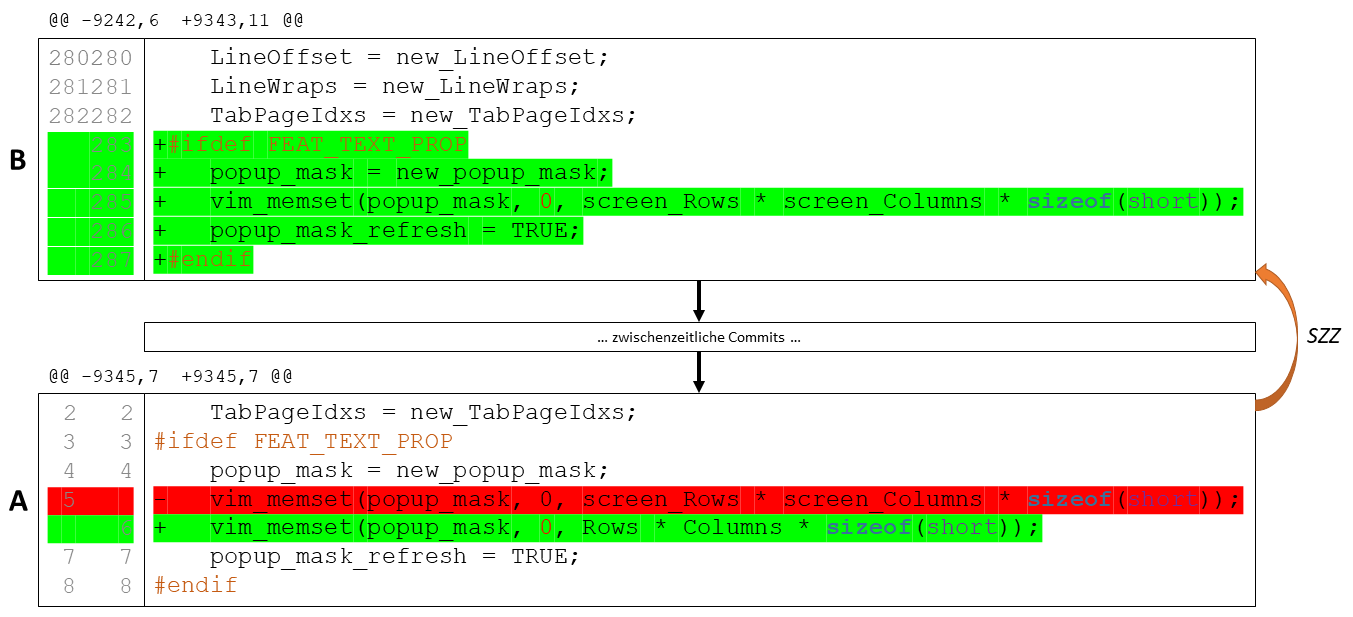
\includegraphics[width=\textwidth]{images/Bug_example_real}
    \caption{Reales Beispiel eines Fehlers mit korrektivem (A) und fehlereinführendem (B) Commit\label{fig:bug-example}}
\end{figure}

Auf Basis der Daten der Haupttabellen können nun die für das Training der Klassifikatoren benötigten Metriken berechnet werden.

\section{Metriken}

Wie bereits in \hyperref[classification]{Abschnitt 2.2} erwähnt wurde, dienen Attribute zur Erlernung der Machine-Learning-Klassifikatoren. Im hier vorliegenden Szenario werden sogenannte Metriken als Attribute verwendet. Bei Metriken handelt sich sich um Zahlenwerte, die Eigenschaften eines Softwareprojekts quantifizieren. Die Metriken werden im hier vorliegenden Fall in die üblichen Kategorien Codemetriken und Prozessmetriken aufgeteilt und jeweils anhand der vorhandenen Rohdaten der Haupttabellen berechnet \cite{Rahman2013}. Codemetriken werden genutzt um Eigenschaften von Sourcecode, wie zum Beispiel \glqq Größe\grqq{} oder Komplexität, zu messen \cite{Rahman2013}. Prozessmetriken dienen hingegen zur Messung von Eigenschaften, die anhand von Metadaten aus Software-Repositories erörtert werden können \cite{Rahman2013}. Beispiele dafür sind die Anzahl der Veränderungen einer bestimmten Datei oder die Anzahl der aktiven Entwickler an einem Projekt. Für diese Arbeit wurden elf featurebasierte Metriken errechnet, aufgeteilt in sieben Prozess- und vier Codemetriken. Fünf der Prozessmetriken wurden aus wissenschaftlichen Arbeiten \cite{Rahman2013,Queiroz2016} entnommen. Die weiteren sechs Metriken wurden auf Basis der von PyDriller erhaltenen Metadaten der Commits berechnet. Eine Auflistung der elf Metriken samt Beschreibungen ist in \autoref{tab:metrics} aufgeführt. Die Berechnung der einzelnen Metriken erfolgte entweder direkt mittels SQL-Abfragen oder kombiniert mittels SQL-Abfragen und Berechnungen durch ein Python-Skript.

\begin{table}[t]
\centering
\caption{Übersicht der berechneten Metriken des featurebasierten Datensets}
\label{tab:metrics}
\resizebox{\linewidth}{!}{%
\begin{tabular}{|l|l|l|c|} 
\cline{2-4}
\multicolumn{1}{l|}{}       & \textbf{Metrik}                                                                                & \textbf{Beschreibung}                                                                                                                                                                                                                                                                                                                              & \textbf{Quelle}   \\ 
\hline
\multirow{7}{*}{\textbf{\parbox[t]{2mm}{\multirow{3}{*}{\rotatebox[origin=c]{90}{Prozessmetriken}}}}} & Anzahl der Commits (COMM)                                                                      & Anzahl der Commits, die dem Feature in einem Release zugeordnet sind.                                                                                                                                                                                                                                                                              & \cite{Rahman2013,Queiroz2016}                  \\ 
\cline{2-4}
                            & \begin{tabular}[c]{@{}l@{}}Anzahl der\\aktiven Entwickler (ADEV) \end{tabular}                 & \begin{tabular}[c]{@{}l@{}}Anzahl der Entwickler, die innerhalb eines Releases das Feature \\bearbeitet (geändert, gelöscht oder hinzugefügt) haben. \end{tabular}                                                                                                                                                                                 & \cite{Rahman2013,Queiroz2016}                  \\ 
\cline{2-4}
                            & \begin{tabular}[c]{@{}l@{}}eindeutige\\Entwickleranzahl (DDEV) \end{tabular}                   & \begin{tabular}[c]{@{}l@{}}kumulierte Anzahl der Entwickler, die innerhalb eines Releases das Feature \\bearbeitet (geändert, gelöscht oder hinzugefügt) haben. \end{tabular}                                                                                                                                                                      & \cite{Rahman2013,Queiroz2016}                  \\ 
\cline{2-4}
                            & \begin{tabular}[c]{@{}l@{}}Erfahrung aller\\Entwickler (EXP) \end{tabular}                     & \begin{tabular}[c]{@{}l@{}}geometrisches Mittel der \glqq Erfahrung\grqq{} aller Entwickler, die innerhalb eines \\Releases das Feature bearbeitet (geändert, gelöscht oder hinzugefügt) haben. \\Erfahrung ist definiert als Summe der geänderten, gelöschten oder\\hinzugefügten~Zeilen in den dem Feature zugeordneten Dateien. \end{tabular} & \cite{Rahman2013,Queiroz2016}                  \\ 
\cline{2-4}
                            & \begin{tabular}[c]{@{}l@{}}Erfahrung des meist \\beteiligten Entwicklers\\(OEXP) \end{tabular} & \begin{tabular}[c]{@{}l@{}}\glqq Erfahrung\grqq{} des Entwicklers, die innerhalb eines Releases das Feature \\am häufigsten bearbeitet (geändert, gelöscht oder hinzugefügt) hat.\\Erfahrung ist definiert als Summe der geänderten, gelöschten oder\\hinzugefügten Zeilen in den dem Feature zugeordneten Dateien. \end{tabular}     & \cite{Rahman2013,Queiroz2016}                  \\ 
\cline{2-4}
                            & \begin{tabular}[c]{@{}l@{}}Grad der\\Änderungen (MODD) \end{tabular}                           & \begin{tabular}[c]{@{}l@{}}Anzahl der Bearbeitungen (Änderung, Entfernung, Erweiterung) des\\Features innerhalb eines Releases. \end{tabular}                                                                                                                                                                                          & *                 \\ 
\cline{2-4}
                            & \begin{tabular}[c]{@{}l@{}}Umfang der\\Änderungen (MODS) \end{tabular}                         & \begin{tabular}[c]{@{}l@{}}Anzahl der bearbeiteten Features innerhalb eines Releases \\(featureübergreifender Wert). Idee: Je mehr Features in einem Release \\ bearbeitet worden sind, desto fehleranfälliger scheinen diese zu sein. \end{tabular}                                                              & *                 \\ 
\hline
\multirow{4}{*}{\textbf{\parbox[t]{2mm}{\multirow{3}{*}{\rotatebox[origin=c]{90}{Codemetriken}}}}} & \begin{tabular}[c]{@{}l@{}}Anzahl der\\Codezeilen (NLOC) \end{tabular}                         & \begin{tabular}[c]{@{}l@{}}Durchschnittliche Anzahl der Codezeilen der dem Feature \\zugeordneten Dateien innerhalb eines Releases. \end{tabular}                                                                                                                                                                                      & *                 \\ 
\cline{2-4}
                            & \begin{tabular}[c]{@{}l@{}}Zyklomatische\\Komplexität (CYCO) \end{tabular}                     & \begin{tabular}[c]{@{}l@{}}Durchschnittliche zyklomatische Komplexität der dem Feature \\zugeordneten Dateien innerhalb eines Releases. \end{tabular}                                                                                                                                                                                  & *                 \\ 
\cline{2-4}
                            & \begin{tabular}[c]{@{}l@{}}Anzahl der\\hinzugefügten Zeilen (ADDL) \end{tabular}               & \begin{tabular}[c]{@{}l@{}}Durchschnittliche Anzahl der hinzugefügten Codezeilen zu\\den dem Feature zugeordneten Dateien innerhalb eines Releases. \end{tabular}                                                                                                                                                                      & *                 \\ 
\cline{2-4}
                            & \begin{tabular}[c]{@{}l@{}}Anzahl der\\entfernten Zeilen (REML) \end{tabular}                  & \begin{tabular}[c]{@{}l@{}}Durchschnittliche Anzahl der gelöschten Codezeilen von\\den dem Feature zugeordneten Dateien innerhalb eines Releases. \end{tabular}                                                                                                                                                   & *                 \\ 
\hline
\multicolumn{4}{|c|}{\begin{tabular}[c]{@{}c@{}}\textit{* Diese Werte wurden auf Basis der mit PyDriller erhaltenen Metadaten berechnet.}\\\textit{Die Berechnung der Metriken auf Feature-Level erfolgte auf Basis der Metadaten der ihnen zugrunde liegenden Dateien.~}\end{tabular}}                                                                                                                                                                                                               \\
\hline
\end{tabular}
}
\end{table}

Im Hinblick auf die im nächsten Kapitel folgende Evaluation des featurebasierten Datensets, wurden zwei weitere Datensets erstellt, um die Auswirkungen der featurebasierten Metriken auf die Vorhersagen der Klassifikatoren vergleichbar zu machen. Beide weiteren Datensets verfolgen einen klassischen dateibasierten Ansatz, wie er in der Machine-Learning-gestützten Fehlererkennung üblich ist und basieren auf die Methodik, die von Moser et al. \cite{Moser2008}, die bereits in \hyperref[moser]{Abschnitt 2.3} vorgestellt wurde. Ebenfalls wurden die 17 Prozessmetriken dieser wissenschaftlichen Arbeit übernommen. Eine Visualisierung zur Unterscheidung der drei Datensets ist in \autoref{fig:dataset} dargestellt.

\begin{figure}[t]
    \centering
    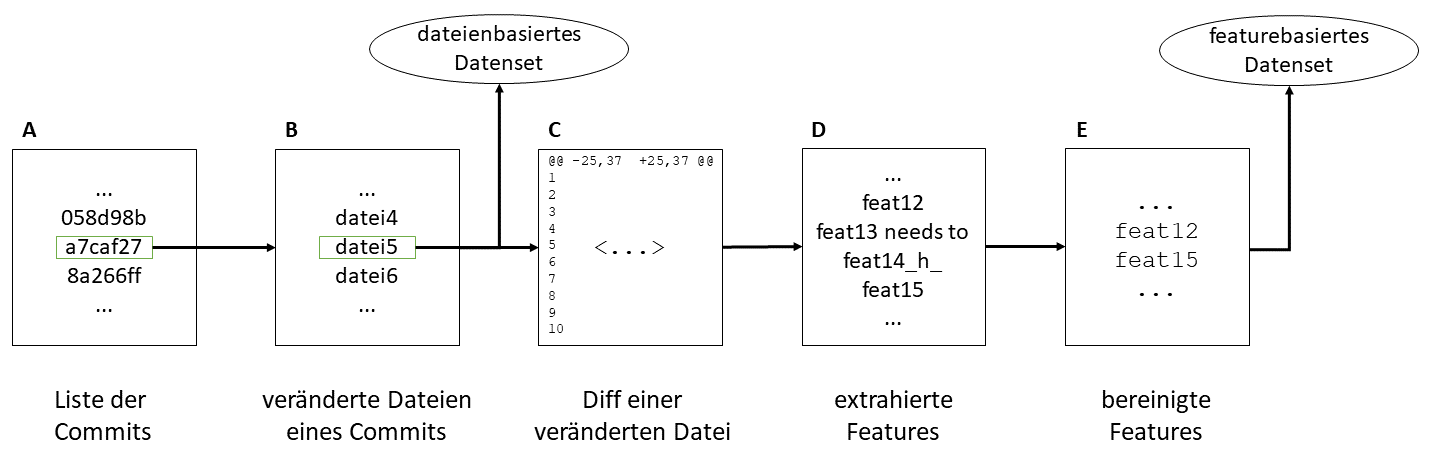
\includegraphics[width=\textwidth]{images/Dataset}
    \caption{Visualisierung zur Unterscheidung der Datensets\label{fig:dataset}}
\end{figure}

Die Abbildung zeigt die Wege der Erstellung des featurebasierten Datensets (Pfad A - G) und der dateibasierten Datensets nach \cite{Moser2008}. Diese unterteilen sich in das \glqq einfache\grqq{} dateibasierte Datenset (Pfad A, B, H, I) und das erweiterte dateibasierte Datenset (Kombination beider Pfade). Die Erstellung des featurebasierten Datensets wurde bereits umfassend bis zu diesem Abschnitt erläutert. Weitere Informationen zur Finalisierung des Datensets folgen im Verlauf dieses Abschnitts.

Die Erstellung der dateibasierten Datensets erfolgt ebenfalls auf Basis der mit PyDriller erhaltenen Rohdaten der Commits der Softwareprojekte und den daraus extrahierten veränderten Dateien (A + B). Es ist somit keine weitere Verarbeitung der Rohdaten nötig. Sie dienen dann als Grundlage zur Berechnung der 17 Metriken (H) nach \cite{Moser2008}. Eine Übersicht der Metriken erfolgte bereits in \hyperref[moser-metrics]{Abschnitt 2.3}. Für die Berechnung der zeitbasierten Metriken \texttt{AAGE} und \texttt{WAGE} mussten die Rohdaten beziehungsweise die in den Rohdaten gelisteten Commits mit ihrem Veröffentlichungsdatum ergänzt werden. Durchgeführt wurde dies ebenfalls mit PyDriller. Als Startpunkt für die Berechnung der vergangenen Wochen wurde jeweils das Datum des ersten Commits eines Releases gewählt.

Das featurebasierte sowie das \glqq einfache\grqq{} Datenset (G + I) bestehen aus den jeweils berechneten feature- (F) und dateibezogenen (H) Metriken sowie den Labeln der Zielklasse. Berechnet werden die Werte der Metriken für die Daten jedes Softwareprojektes. Die daraus resultierenden Tabellen enthalten als Spalten die Werte der elf beziehungsweise 17 Metriken sowie das Label (Zielklasse) \glqq defekt\grqq{} oder \glqq fehlerfrei\grqq{} und als Zeilen die Features bzw. Dateien aggregiert nach Release. Dies bedeutet, dass für den Fall, dass ein Feature oder eine Datei in einem Release mehrfach bearbeitet wurden (d.h. es wird in mehreren Commits bearbeitet), der Durchschnittswert der jeweiligen Metriken innerhalb des Releases berechnet und gespeichert wird. Das Verfahren zur Bestimmung des Labels erfolgt für jede Veränderung eines Features beziehungsweise einer Datei anhand des folgenden Musters:

\begin{table}[H]
\centering
\resizebox{\linewidth}{!}{%
\begin{tabular}{>{\hspace{0pt}}p{0.428\linewidth}>{\hspace{0pt}}p{0.046\linewidth}>{\hspace{0pt}}p{0.283\linewidth}>{\hspace{0pt}}p{0.046\linewidth}>{\hspace{0pt}}p{0.187\linewidth}}
fehlereinführend       & + & korrektiv       & = & defekt      \\
fehlereinführend       & + & nicht korrektiv & = & defekt      \\
nicht fehlereinführend & + & korrektiv       & = & fehlerfrei  \\
nicht fehlereinführend & + & nicht korrektiv & = & fehlerfrei 
\end{tabular}
}
\end{table}

Die Informationen zum Status eines Features basieren dabei auf den ihm zugrundliegenden Dateien. Für den Fall, dass ein Feature oder eine Datei mehrfach innerhalb eines Releases bearbeitet sein sollte, erfolgt die Bestimmung des Labels anhand der folgenden Regeln:

\begin{itemize}
\setlength{\itemsep}{-2pt}
\item im Fall von Features wird überprüft, ob innerhalb des Releases das Feature mindestens ein Mal als \glqq defekt\grqq{} markiert wurde. Ist dies der Fall, so wird angenommen, dass das Feature in dem betreffenden Release defekt ist. Tritt dieser Fall nicht ein, so gilt das Feature als fehlerfrei.
\item im Fall von Dateien wird der jeweils letzte Commit der Dateien im betreffenden Release überprüft. Ist die Datei dort als \glqq fehlerfrei\grqq{} markiert, so wird angenommen, dass sie fehlerfrei ist. Ist sie als \glqq defekt\grqq{} markiert, so wird angenommen, dass sie in diesem Release defekt ist.
\end{itemize}

Die so erstellten einzelnen Tabellen werden anschließend zu jeweils einer gemeinsamen Tabelle konkateniert, sodass eine umfangreiche Auflistung an Metriken inklusive der zugehörigen Labels entsteht. Diese Auflistung gibt an, welche Charakteristika ein Feature beziehungsweise eine Datei aufweisen muss, um als \glqq fehlerfrei\grqq{} oder \glqq defekt\grqq{} eingestuft zu werden und dient als Lerngrundlage der Klassifikatoren für zukünftige Vorhersagen.

Eine Besonderheit stellt das zweite für den Vergleich im Rahmen der Evaluation erstellte dateibasierte Datenset dar (J). Es basiert auf dem \glqq einfachen\grqq{} Datenset (I) mit den Metriken aus \cite{Moser2008}, umfasst aber zusätzlich die elf Metriken des featurebasierten Datensets (G) aus \autoref{tab:metrics}. Dazu wurden die Werte der featurebasierten Metriken auf Dateiebene \glqq gemapped\grqq{} beziehungsweise übertragen. Dies bedeutetet, dass für jede im dateibasierte Datenset referenzierte Datei eines Releases analysiert wurde, welche Features in der jeweiligen Datei erwähnt wurde. Von diesen Features wurden dann die zugehörigen Metriken des featurebasierten Datensets ermittelt und der Durchschnittswert berechnet um im erteiterten Datenset eingetragen. Sollte in einer Datei keine Features erwähnt worden sein, so wird für die featurebasierten Metriken jeweils der Wert 0 gespeichert. Wie zu Beginn des Abschnitts erwähnt wurde, kann auf diesem Weg das featurebasierte Datenset mit einem klassischen dateibasierten Datenset verglichen werden, da die Bedingungen für den Vergleich geschaffen wurden. Ein direkter Vergleich zwischen den verschiedenen Datensets ist aus den genannten Gründen nicht praktikabel.

Die auf die zuvor beschriebene Weise erstellten Datensets können nun zur Erlernung der Klassifikatoren verwendet werden. Dieser Vorgang wird im kommenden Kapitel erläutert.

\fbox{\parbox{\linewidth}{RQ1b: WIE WEIT MÜSSEN DIE DATEN VORVERARBEITET WERDEN, UM SIE FÜR DAS TRAINING NUTZBAR ZU MACHEN?\medskip\\
Eine umfassende Vorverarbeitung der Daten aus den Repositories ist nicht nötig. Die Verarbeitungsschritte bestanden aus: Extraktion der Features inklusive Bereinigung, Identifizierung von korrektiven Commits mittels Analyse der Commit-Nachrichten, Analyse nach fehlereinführenden Commits unter Zuhilfenahme des SZZ-Algorithmus sowie Berechnung von elf Metriken, welche als Attribute für die Erlernung der Klassifikatoren dienen.}}

\cleardoublepage

%\begin{table}
%\centering
%\caption{Overview of used metrics}
%\label{tab:metrics}
%\resizebox{\linewidth}{!}{%
%\begin{tabular}{l|llc} 
%\cline{2-4}
%                             & \textbf{Metric}                                                                            & \textbf{Description}                                                                                                                                                                                                                                                                                        & \multicolumn{1}{c|}{\textbf{Source} }  \\ 
%\hline
%\multirow{7}{*}{\textbf{\rotatebox[origin=c]{90}{Process metrics}}} & Number of commits (COMM)                                                                   & Number of commits associated with the feature/file in a release.                                                                                                                                                                                                                                             & \cite{Rahman2013,Queiroz2016}                                    \\
%                             & Number of active developers (ADEV)                                                         & \begin{tabular}[c]{@{}l@{}}Number of developers who have edited (changed, deleted or added) \\the feature / file within a release\end{tabular}                                                                                                                                                               & \cite{Rahman2013,Queiroz2016}                                    \\
%                             & Number of distinct developers (DDEV)                                                       & \begin{tabular}[c]{@{}l@{}}Cumultative number of developers who have edited (changed, deleted or added) \\the feature / file within a release\end{tabular}                                                                                                                                                   & \cite{Rahman2013,Queiroz2016}                                    \\
%                             & Experience of all develepoers (EXP)                                                        & \begin{tabular}[c]{@{}l@{}}geometric mean of the experience of all developers who have edited \\(changed, deleted or added) the feature / file within a release.~\\Experience is defined as the sum of the changed, deleted or added \\lines in the commits associated with the feature / file.\end{tabular} & \cite{Rahman2013,Queiroz2016}                                    \\
%                             & \begin{tabular}[c]{@{}l@{}}Experience of the most involved developers\\(OEXP)\end{tabular} & \begin{tabular}[c]{@{}l@{}}Experience of the developer who has edited (changed, deleted or added) \\the feature / file most often within a release. Experience is defined as the \\sum of changed, deleted, or added lines in the commits associated with the \\feature/file.\end{tabular}                   & \cite{Rahman2013,Queiroz2016}                                    \\
%                             & Degree of modifications (MODD)                                                             & Number of edits (change, removal, extension) of the feature / file within a release.                                                                                                                                                                                                                         & new                                    \\
%                             & Scope of modifications (MODS)                                                              & \begin{tabular}[c]{@{}l@{}}Number of edited features / files within a release (feature or file overlapping value). \\Idea: The more features / files have been edited in a release, \\the more error-prone they seem to be.\end{tabular}                                                                     & new                                    \\ 
%\hline
%\multirow{4}{*}{\textbf{\rotatebox[origin=c]{90}{Code metrics}}} & Lines of code (NLOC)                                                                       & \begin{tabular}[c]{@{}l@{}}Average number of lines of code of the files associated with the feature /\\~file within a release.\end{tabular}                                                                                                                                                                  & new                                    \\
%                             & Cyclomatic Complexity (CYCO)                                                               & \begin{tabular}[c]{@{}l@{}}Average cyclomatic complexity of the files associated with the feature / \\file within a release.\end{tabular}                                                                                                                                                                    & new                                    \\
%                             & Number of added lines (ADDL)                                                               & \begin{tabular}[c]{@{}l@{}}Average number of lines of code added to the files associated with \\the feature / file within a release.\end{tabular}                                                                                                                                                            & new                                    \\
%                             & Number of removed lines (REML)                                                             & \begin{tabular}[c]{@{}l@{}}Average number of lines of code deleted from the files associated \\with the feature / from the file within a release\end{tabular}                                                                                                                                                & new                                   
%\end{tabular}
%}
%\end{table}
%
%\begin{table}[]
%\caption{Übersicht des Schemas der Metrics-Tabellen des Datensets}
%\label{tab:schema2}
%\resizebox{\textwidth}{!}{%
%\begin{tabular}{ll|ll}
%\textbf{Spaltenname} & \textbf{Beschreibung}                                                                                                                                                                          & \textbf{Spaltenname} & \textbf{Beschreibung}                                                                                                                                                           \\ \hline
%name                 & Name des Softwareprojekts                                                                                                                                                                      & oexp                 & \begin{tabular}[c]{@{}l@{}}"Erfahrung" des Entwicklers, der am\\ meisten zum betreffenden Feature / \\ zur betreffenden Datei in  einem Release \\ beigetragen hat\end{tabular} \\
%release\_number      & \begin{tabular}[c]{@{}l@{}}zugehörige Release-Version\\ basierend auf vergebene Tags\end{tabular}                                                                                              & scat                 & \begin{tabular}[c]{@{}l@{}}Scattering Degree des betreffenden Features / \\ der betreffenden Datei\end{tabular}                                                                 \\
%feature / filename   & \begin{tabular}[c]{@{}l@{}}betreffendes Feature / \\ betreffende Datei\end{tabular}                                                                                                            & tang                 & \begin{tabular}[c]{@{}l@{}}Tangling Degree des betreffenden Features / \\ der betreffenden Datei\end{tabular}                                                                   \\
%comm                 & \begin{tabular}[c]{@{}l@{}}Anzahl der Commits, die in einem\\ Release dem betreffenden Feature / \\ der betroffenen Datei gewidmet sind\end{tabular}                                           & nloc                 & \begin{tabular}[c]{@{}l@{}}Durchschnittliche Lines of Code der Bearbeitungen \\ des betreffenden Features / der betreffenden Datei\\ in einem Release\end{tabular}              \\
%adev                 & \begin{tabular}[c]{@{}l@{}}Anzahl der Entwickler, die das\\ betreffende Feature / die betreffende \\ Datei in einem Release bearbeitet haben\end{tabular}                                      & cyco                 & \begin{tabular}[c]{@{}l@{}}Durchschnittliche zyklomatische Komplexität der \\ Bearbeitungen  des betreffenden Features /\\ der betreffenden Datei in einem Release\end{tabular} \\
%ddev                 & \begin{tabular}[c]{@{}l@{}}kummulierte Anzahl der Entwickler, \\ die das betreffende Feature / \\ die betreffende Datei in einem\\ Release bearbeitet haben\end{tabular}                       & addl                 & \begin{tabular}[c]{@{}l@{}}Durchschnittliche Anzahl der hinzugefügten Zeilen \\ des betreffenden Features / der betreffenden Datei\\ in einem Release\end{tabular}              \\
%exp                  & \begin{tabular}[c]{@{}l@{}}Geometrisches Mittel der "Erfahrung"\\ aller Entwickler, die am betreffenden\\ Feature / an der betreffenden Datei\\ in einem Release gearbeitet haben\end{tabular} & reml                 & \begin{tabular}[c]{@{}l@{}}Durchschnittliche Anzahl der entfernten Zeilen \\ des betreffenden Features / der betreffenden Datei\\ in einem Release\end{tabular}                
%\end{tabular}%
%}
%\end{table}